\documentclass[tikz,border=3pt]{standalone}
\usepackage{pgfplots}
\pgfplotsset{compat=1.17}
\definecolor{pdcsblue}{RGB}{0,114,178}
\definecolor{pdcsorange}{RGB}{213,94,0}
\begin{document}
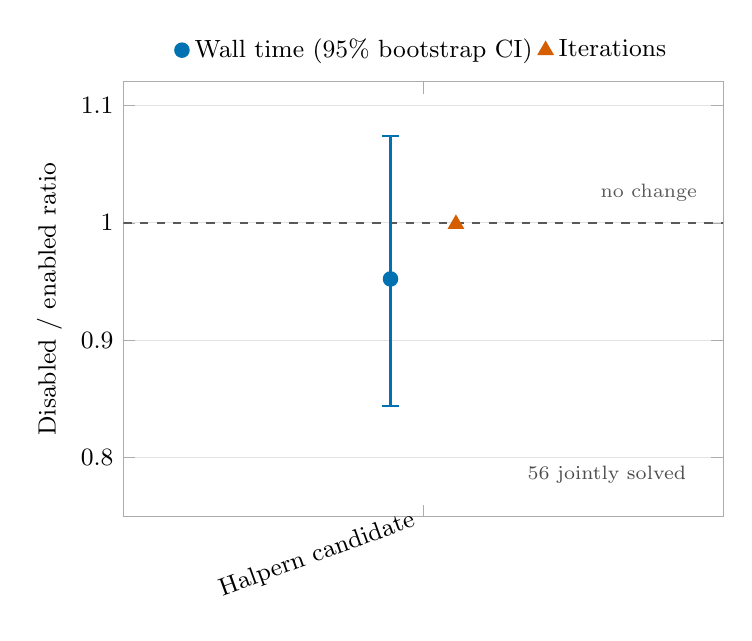
\begin{tikzpicture}
\begin{axis}[
  width=9.2cm,
  height=7.1cm,
  % no title
  title style={font=\small},
  xmin=0.45,
  xmax=1.55,
  ymin=0.75,
  ymax=1.12,
  xtick={1},
  xticklabels={Halpern candidate},
  xticklabel style={rotate=20,anchor=east,font=\small},
  ytick={0.8,0.9,1,1.1},
  ylabel={Disabled / enabled ratio},
  tick label style={font=\small},
  label style={font=\small},
  legend style={
    at={(0.5,1.02)},
    anchor=south,
    legend columns=2,
    draw=none,
    font=\small
  },
  ymajorgrids=true,
  grid style={gray!22},
  axis line style={gray!65},
  tick style={gray!65},
]
\addplot[black!65,dashed,line width=0.8pt,forget plot]
  coordinates {(0.45,1) (1.55,1)};
\node[anchor=south east,font=\scriptsize,text=black!65]
  at (axis cs:1.52,1.01) {no change};

\addplot+[
  only marks,
  mark=*,
  mark size=2.6pt,
  color=pdcsblue,
  mark options={fill=pdcsblue},
  error bars/.cd,
  y dir=both,
  y explicit,
  error bar style={line width=0.85pt},
  error mark options={rotate=90,mark size=3pt,line width=0.85pt},
] coordinates {
  (0.94,0.95220307) += (0,0.12178083) -= (0,0.10841743)
};
\addlegendentry{Wall time (95\% bootstrap CI)}

\addplot+[
  only marks,
  mark=triangle*,
  mark size=3.1pt,
  color=pdcsorange,
  mark options={fill=pdcsorange},
] coordinates {
  (1.06,0.99892883)
};
\addlegendentry{Iterations}
\node[anchor=south east,font=\scriptsize,text=black!70] at (axis cs:1.50,0.77) {56 jointly solved};
\end{axis}
\end{tikzpicture}
\end{document}
